% Copyright 2004 by Till Tantau <tantau@users.sourceforge.net>.
%
% In principle, this file can be redistributed and/or modified under
% the terms of the GNU Public License, version 2.
%
% However, this file is supposed to be a template to be modified
% for your own needs. For this reason, if you use this file as a
% template and not specifically distribute it as part of a another
% package/program, I grant the extra permission to freely copy and
% modify this file as you see fit and even to delete this copyright
% notice. 

% \UseRawInputEncoding
\documentclass{beamer}

% There are many different themes available for Beamer. A comprehensive
% list with examples is given here:
% http://deic.uab.es/~iblanes/beamer_gallery/index_by_theme.html
% You can uncomment the themes below if you would like to use a different
% one:
%\usetheme{AnnArbor}
%\usetheme{Antibes}
%\usetheme{Bergen}
%\usetheme{Berkeley}
%\usetheme{Berlin}
%\usetheme{Boadilla}
%\usetheme{boxes}
%\usetheme{CambridgeUS}
%\usetheme{Copenhagen}
%\usetheme{Darmstadt}
%\usetheme{default}
%\usetheme{Frankfurt}
%\usetheme{Goettingen}
%\usetheme{Hannover}
%\usetheme{Ilmenau}
%\usetheme{JuanLesPins}
%\usetheme{Luebeck}
\usetheme{Madrid}
%\usetheme{Malmoe}
%\usetheme{Marburg}
%\usetheme{Montpellier}
%\usetheme{PaloAlto}
%\usetheme{Pittsburgh}
%\usetheme{Rochester}
%\usetheme{Singapore}
%\usetheme{Szeged}
%\usetheme{Warsaw}

\usepackage{pgfgantt}
\usepackage{todonotes}
\usepackage{media9}
\usepackage{fontawesome5}
\usepackage{subfigure}
\usepackage{booktabs,array}
\usepackage{tabulary}
\usepackage{caption}
\usepackage{graphicx}
\usepackage{siunitx}
\usepackage{arydshln}
\usepackage{multicol}

\usepackage[ruled, vlined, linesnumbered]{algorithm2e} % For algorithms

\usepackage{amsmath} % For typesetting math

% Customize Warsaw color 
\setbeamercolor*{palette primary}{use=structure,fg=white,bg=red!50!black}
\setbeamercolor*{palette secondary}{use=structure,fg=white,bg=red!60!black}
\setbeamercolor*{palette tertiary}{use=structure,fg=white,bg=red!70!black}

% Customize Warsaw block title and background colors
\setbeamercolor{block title}{bg=red!50!black,fg=white}

\setbeamertemplate{bibliography item}{\insertbiblabel}  % insert bibliography numbers instead of symbol
\setbeamertemplate{caption}[numbered] % adds the figure or table number to the caption.


\title[HIL Plant Modeling]{Hardware-in-the-Loop Plant Modeling for Autonomous
  Vehicle}

% % A subtitle is optional and this may be deleted
\subtitle{Progress Presentation}

\author[H.~Grady, N.~Nauman]{Hannah~Grady \and Nicholas~Nauman 
\linebreak Advisor:~Dr.~Suruz~Miah}
% - Give the names in the same order as the appear in the paper.
% - Use the \inst{?} command only if the authors have different
%   affiliation.

\institute[Bradley University] % (optional, but mostly needed)
{
  Department of Electrical and Computer Engineering\\
  Bradley University\\
  1501 W. Bradley Avenue\\
  Peoria, IL, 61625, USA
}
% - Use the \inst command only if there are several affiliations.
% - Keep it simple, no one is interested in your street address.

\date[March~1,~2022]{Tuesday, March~1,~2022}

% - Either use conference name or its abbreviation.
% - Not really informative to the audience, more for people (including
%   yourself) who are reading the slides online

\logo{\hfill\href{http://www.bradley.edu}{
\includegraphics[width=0.75cm]{figs/logoBU1-Print}}}  % place logo in every page 


% \subject{Mobile Robot Localization}
% This is only inserted into the PDF information catalog. Can be left
% out. 

% If you have a file called "university-logo-filename.xxx", where xxx
% is a graphic format that can be processed by latex or pdflatex,
% resp., then you can add a logo as follows:

% \pgfdeclareimage[height=0.5cm]{university-logo}{university-logo-filename}
% \logo{\pgfuseimage{university-logo}}

% Delete this, if you do not want the table of contents to pop up at
% the beginning of each subsection:
\AtBeginSubsection[]
{
  \begin{frame}<beamer>{Outline}
    \tableofcontents[currentsection,currentsubsection]
  \end{frame}
}

% Delete this, if you do not want the table of contents to pop up at
% the beginning of each section:
\AtBeginSection[]
{
  \begin{frame}<beamer>{Outline}
    \tableofcontents[currentsection]
  \end{frame}
}

% Let's get started
\begin{document}

\begin{frame}
  \titlepage
\end{frame}

\begin{frame}{Outline} 
  \tableofcontents%[pausesections]
  % You might wish to add the option [pausesections]
\end{frame}

% Section and subsections will appear in the presentation overview
% and table of contents.
\section{Introduction}

\begin{frame}{Introduction}{}
    \begin{block}{}
    	\begin{itemize}
    		\item Modeled
			\begin{itemize}
				\item Steering Subsystem
    				\item Acceleration Pedal Subsystem
    				\item Brake Pedal Subsystem
			\end{itemize}			    			
    		\item Not Modeled
			\begin{itemize}
				\item Shift Subsystem
    				\item Speed Subsystem
    				\item Speed Control Subsystem
			\end{itemize}			    			
    		\item Manual Data vs. By-Wire Data
    		\item Neural Network Modeling \cite{Zhou2019} \cite{matlabNeuralNet}
		\end{itemize}
    \end{block}
        
\end{frame}


%----------------------------------

\section{Steering Subsystem}

\begin{frame}{Steering Subsystem}
	\begin{block}{}
  		\begin{figure}[H]
  			\centering 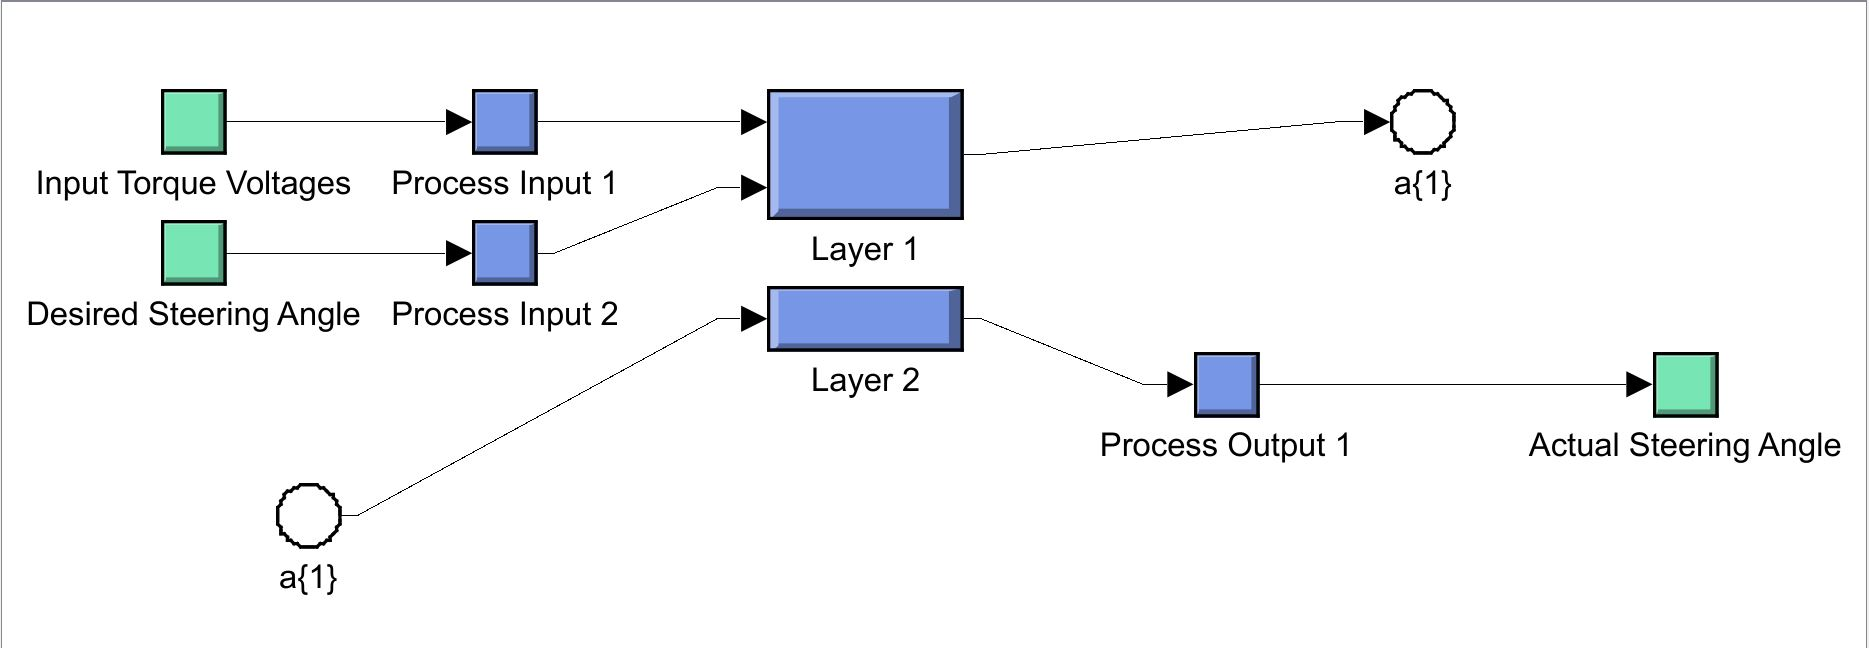
\includegraphics[width=.45\linewidth , height=.37\textheight]{figs/img/steeringSimulinkBlock.jpg}\quad%
			\centering \begin{minipage}[b][0.4\textheight][c]{.45\linewidth}  \begin{itemize}
			\item Only a few samples are just outside of the accuracy requirements
			\item Transfer function model did not meet the accuracy requirements
			\end{itemize} \end{minipage}\\[1em]
			\centering 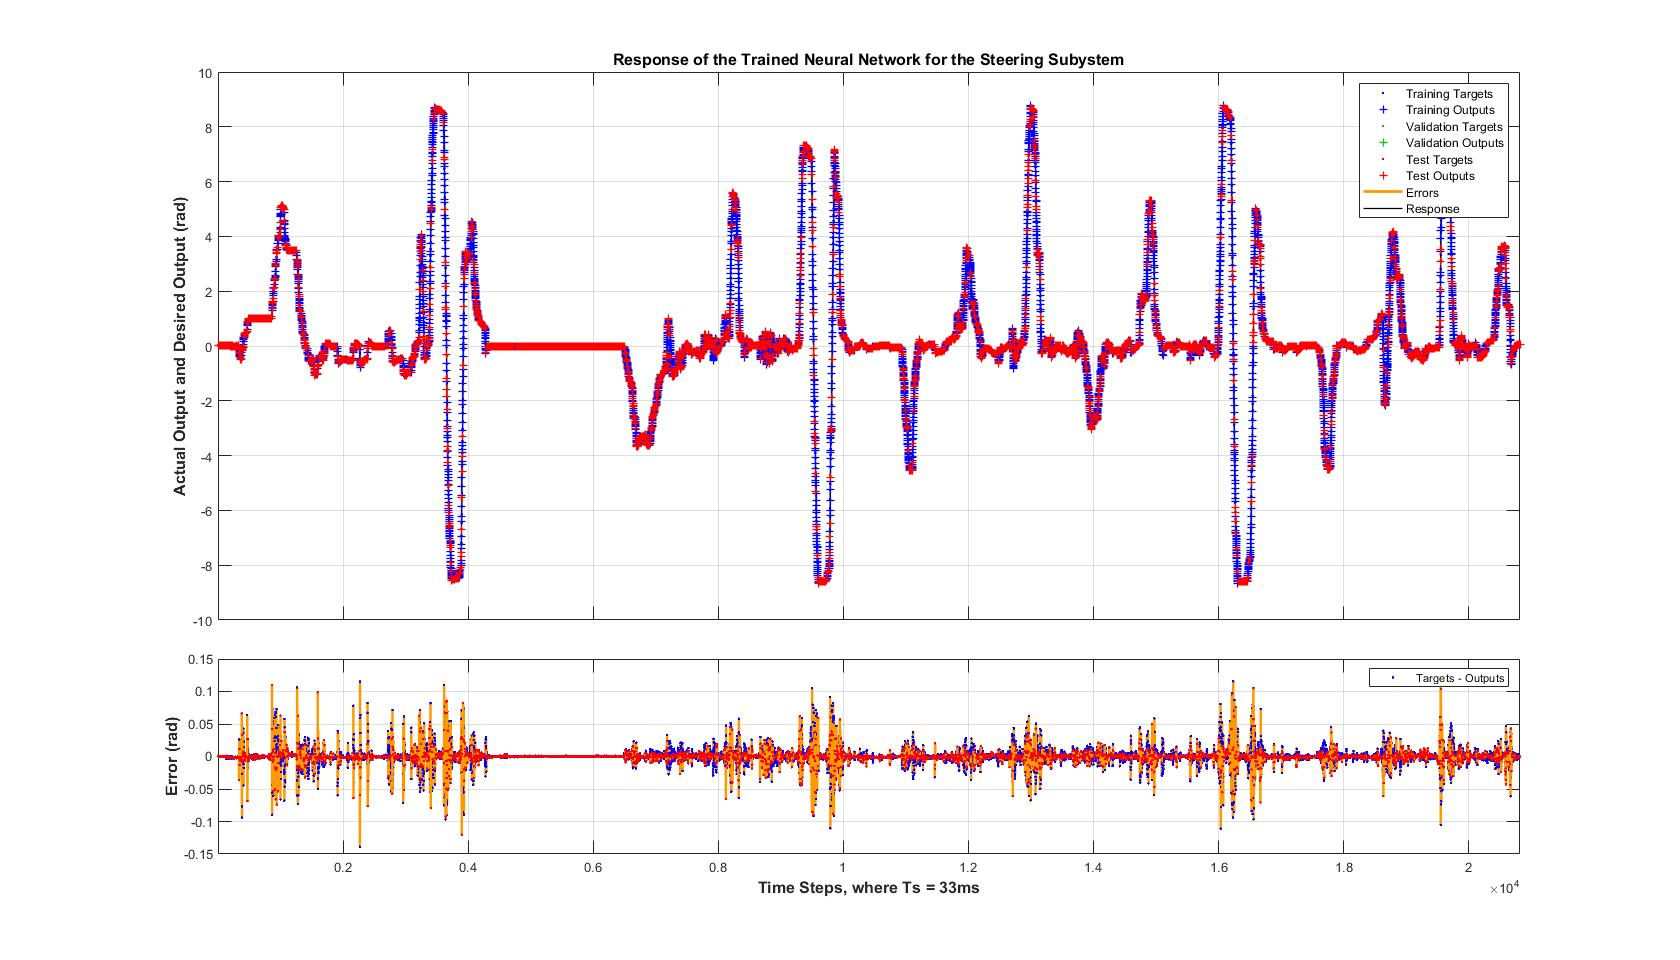
\includegraphics[width=.45\linewidth , height=.37\textheight]{figs/img/steeringNeuralNetworkTrainedOutput.jpg}\quad%
			\centering 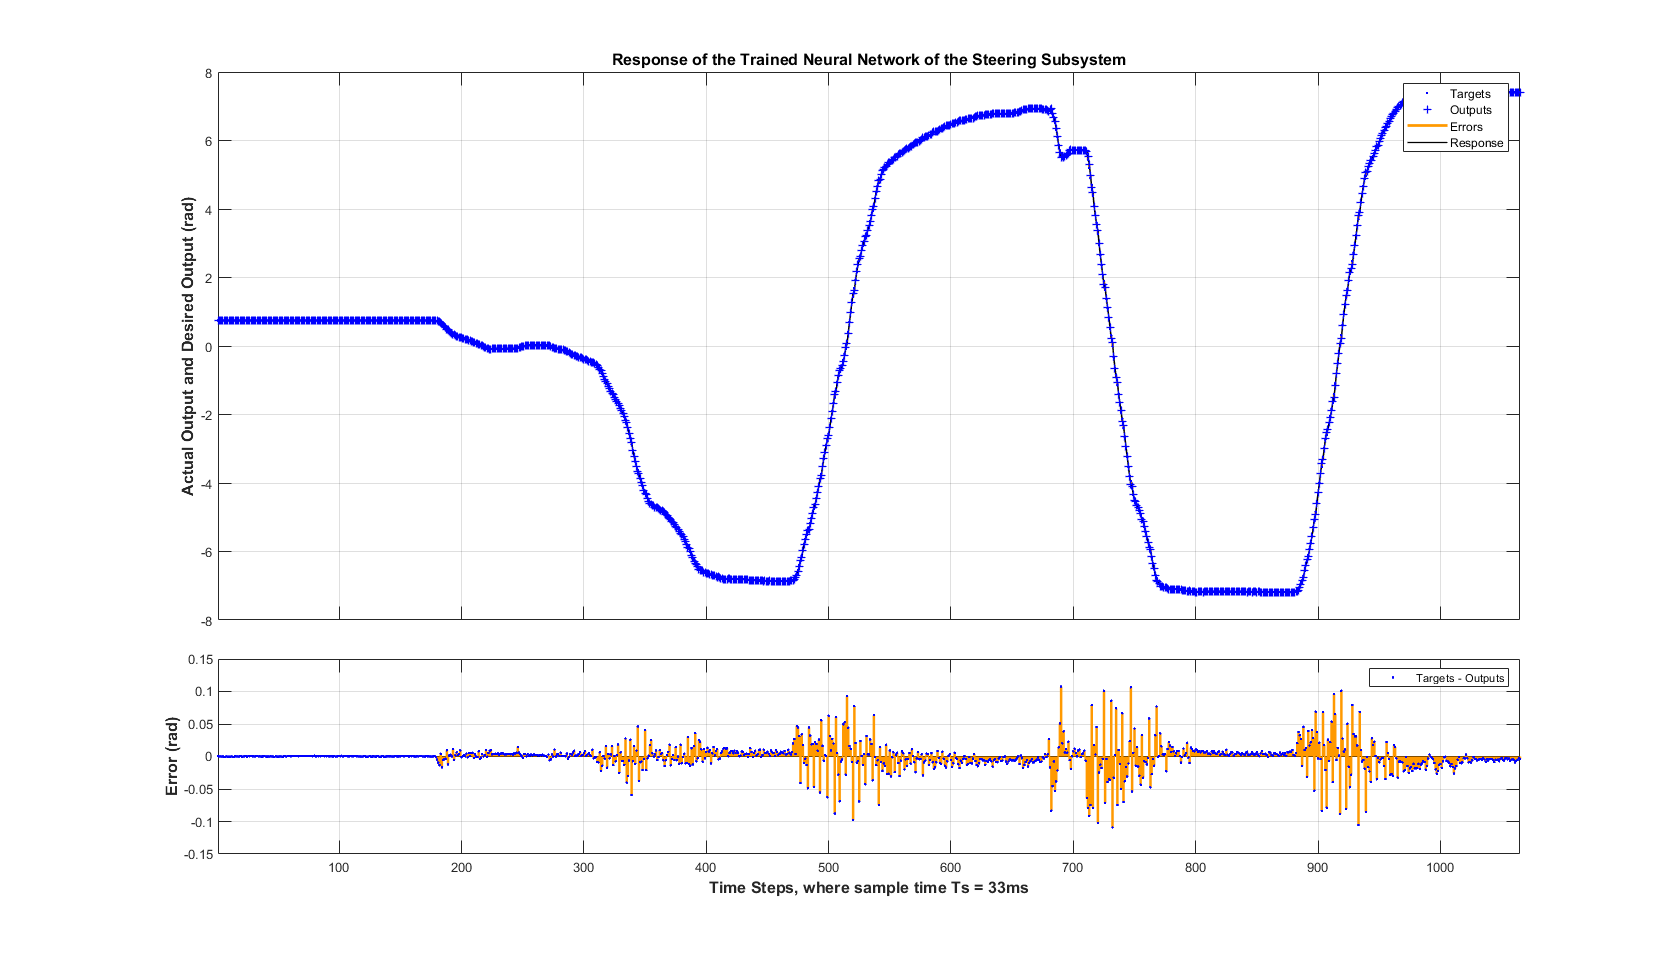
\includegraphics[width=.45\linewidth , height=.37\textheight]{figs/img/steeringNeuralNetworkTrainedOutput2.jpg}
  		\end{figure}
	\end{block}
\end{frame}


%----------------------------------

\section{Acceleration Subsystem}

\begin{frame}{Acceleration Subsystem}
	\begin{block}{}
  		\begin{figure}[H]
  			\centering 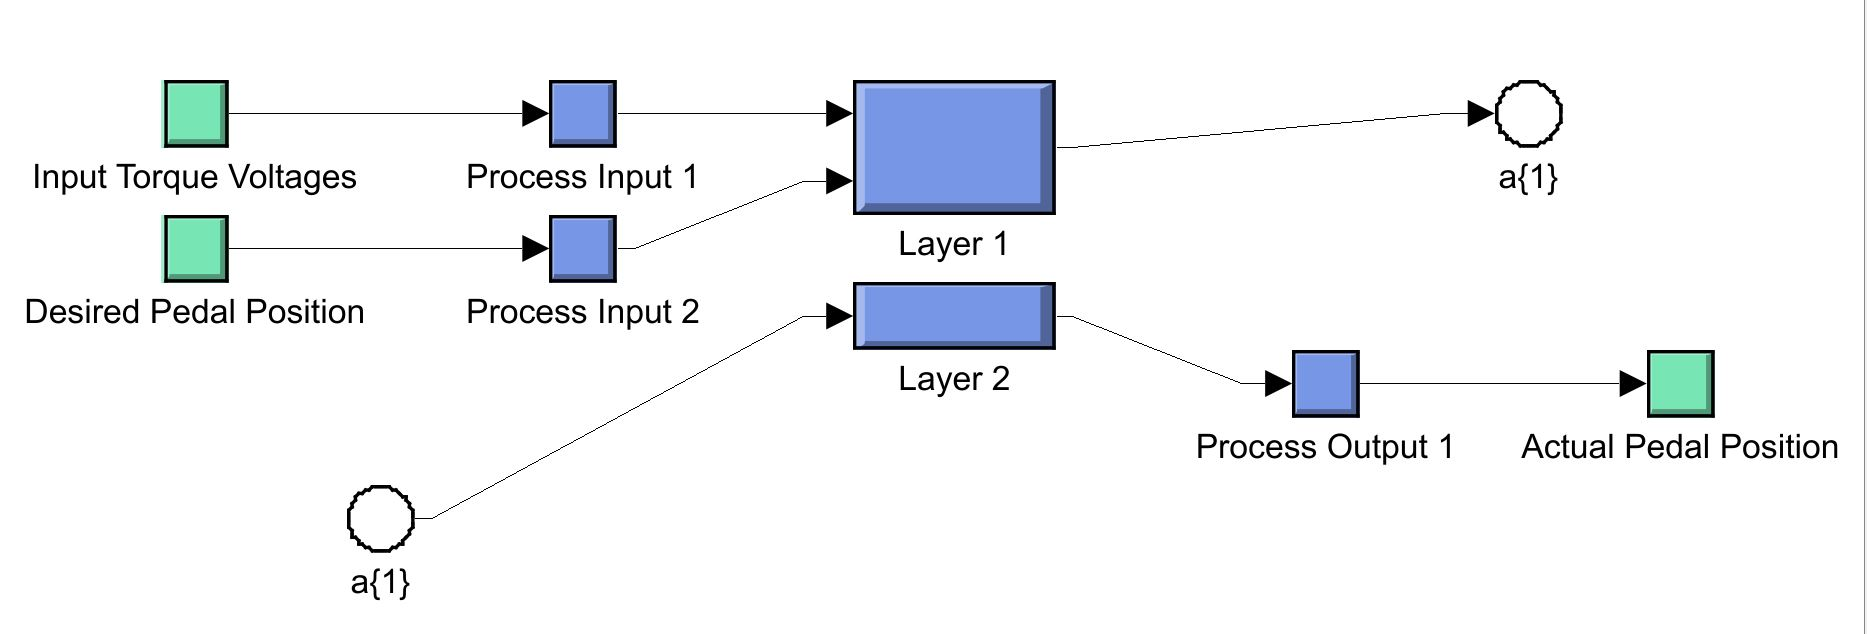
\includegraphics[width=.45\linewidth , height=.37\textheight]{figs/img/accelerationSimulinkBlock.jpg}\quad%
			\centering \begin{minipage}[b][0.4\textheight][c]{.45\linewidth}  \begin{itemize}
			\item All samples within 2\% of the actual output
			\item Transfer function model did not have the same accuracy bounds
			\item Fewer concerns about connections in Simulink
			\end{itemize} \end{minipage}\\[1em]
			\centering 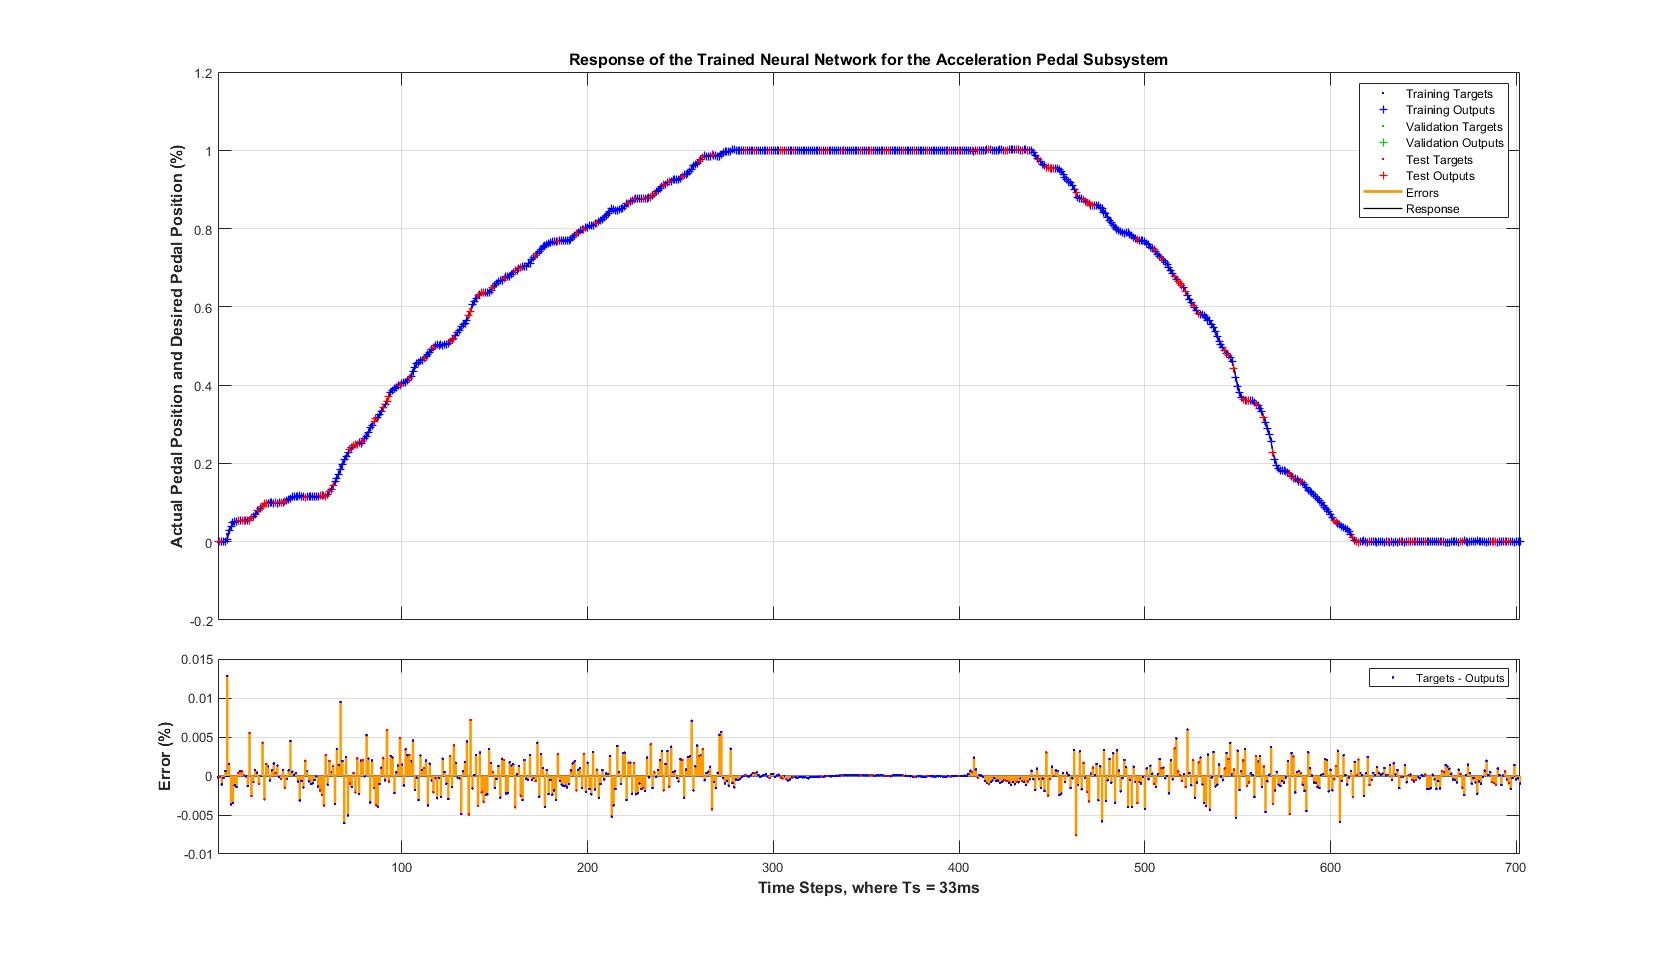
\includegraphics[width=.45\linewidth , height=.37\textheight]{figs/img/accelNeuralNetworkTrainedOutput.jpg}\quad%
			\centering 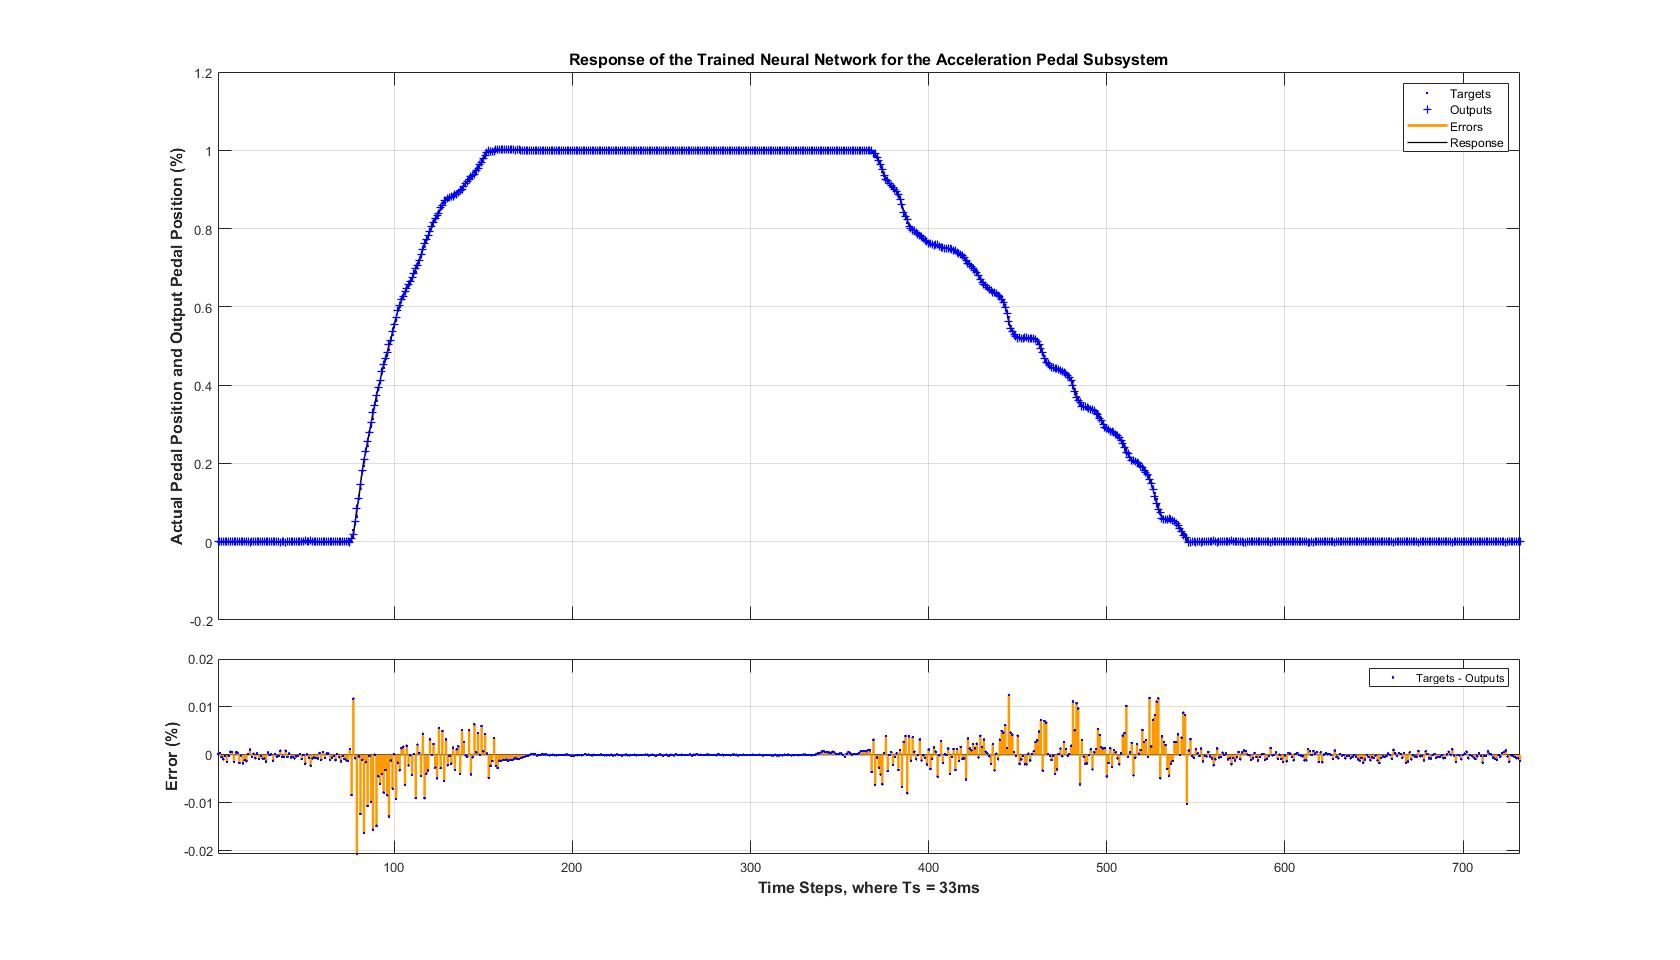
\includegraphics[width=.45\linewidth , height=.37\textheight]{figs/img/accelNeuralNetworkTrainedOutput2.jpg}
  		\end{figure}
	\end{block}
\end{frame}

%--------------------------------

\section{Brake Subsystem}

\begin{frame}{Brake Subsystem}
  \begin{block}{}
\begin{figure}[H]
  			\centering 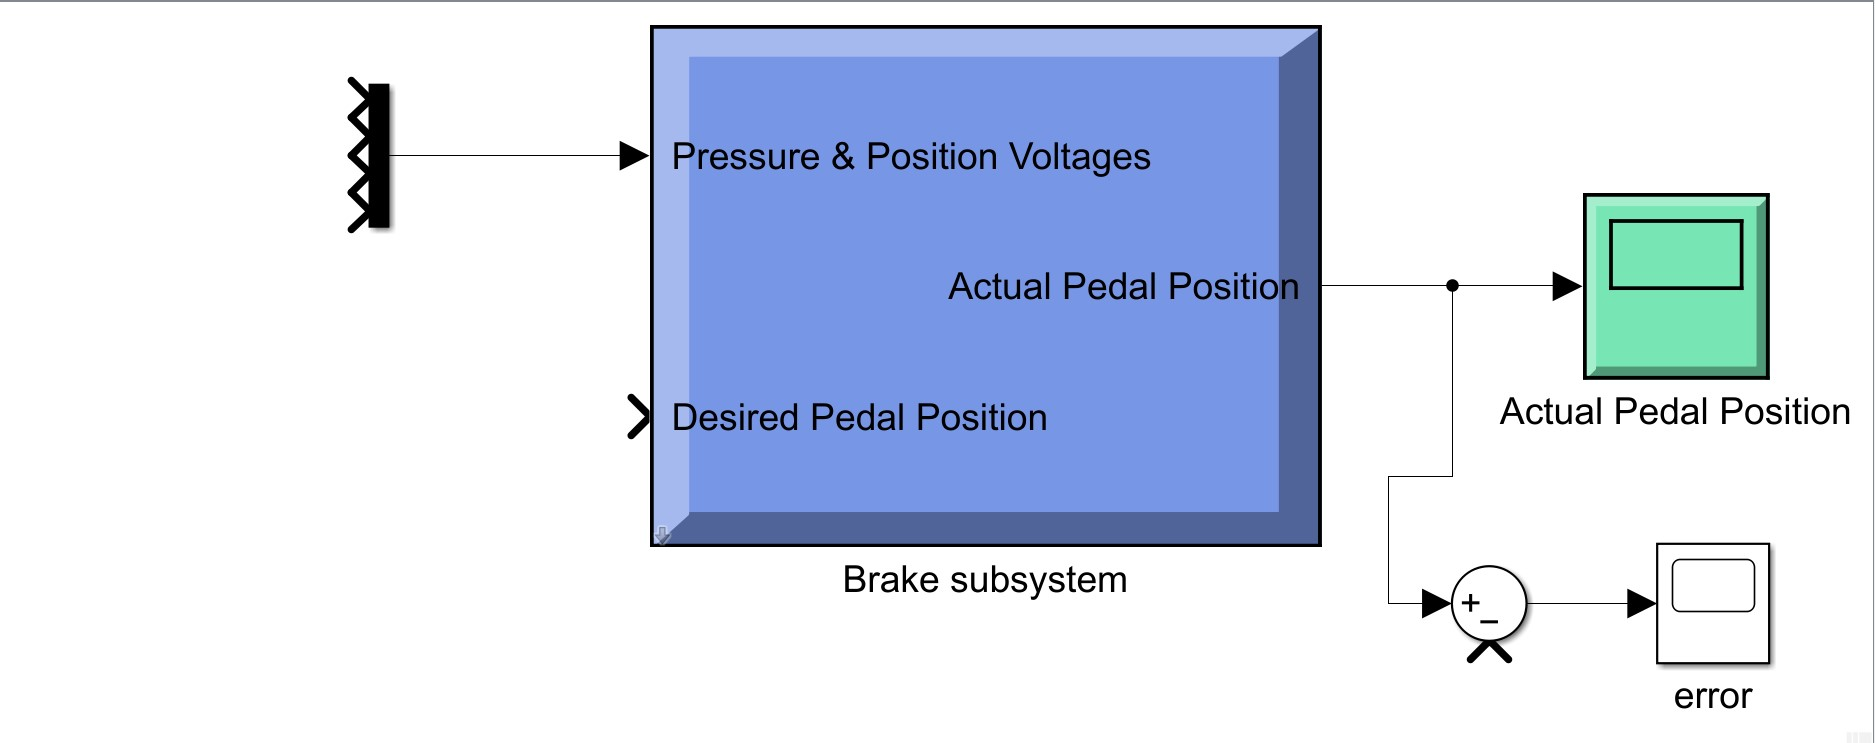
\includegraphics[width=.48\linewidth , height=.37\textheight]{figs/img/newBrakeSimulinkBlock.jpg}\quad%
			\centering \begin{minipage}[b][0.4\textheight][c]{.45\linewidth}  \begin{itemize}
			\item With this model, the error is kept below 5\%
			\item Able to easily track model performance
			\item Provides better results than the transfer function model
			\end{itemize} \end{minipage}\\[1em]
			\centering 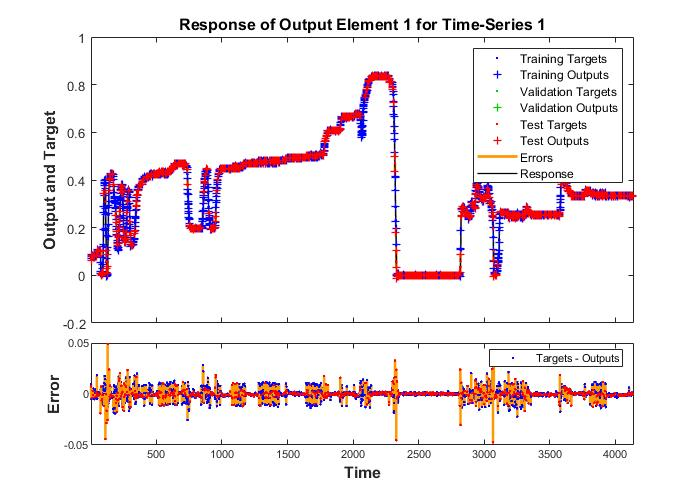
\includegraphics[width=.45\linewidth , height=.37\textheight]{figs/img/brake_new_neuralNetworkFig.jpg}\quad%
			\centering 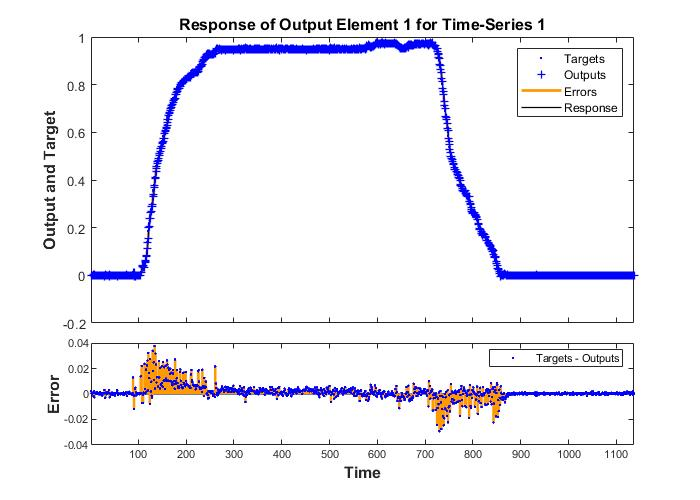
\includegraphics[width=.45\linewidth , height=.37\textheight]{figs/img/brake_new_neuralNetworkFigLog2Test.jpg}
  		\end{figure}
	
  \end{block}

\end{frame}


%----------------------------------


\section{Concluding Remarks}
\begin{frame}{Concluding Remarks}
  \begin{block}{Semester goals}
      \begin{itemize}
        \item Test our modeled subsystems on the HIL bench
        \item Collect data for the remaining subsystems
        \item Model the remaining subsystems and test on the HIL bench
        \item Create final report highlighting our findings
        \item Present our findings
      \end{itemize}
  \end{block}
  \begin{block}{Anticipated Challenges}
      \begin{itemize}
      	\item Having time to model the remaining subsystems
      	\item Needing to correct any models
      \end{itemize}
  \end{block}
\end{frame}

%----------------------------------

\section{References}
\begin{frame}[allowframebreaks]{References}

  \bibliographystyle{IEEEtran}
  \bibliography{bib/references.bib}

\end{frame}


\end{document}



%%% Local Variables:
%%% mode: latex
%%% TeX-master: t
%%% End:
